\newpage
\section{Problem F 稻妻灯谜}
{ \limitfont{}
Input file: standard input \par
Output file: standard output \par
Time limit: 1000ms \par
Memory limit: 512MB \par
}
\subsection*{题目描述}

在稻妻有一种灯谜游戏。有 $n$ 个正四棱柱,每个正四棱柱有 $4$ 个侧面,有一个旋转轴,旋转轴通过上底面的中心和下底面的中心,从上往下看可以绕旋转轴顺时针方向旋转。$4$ 个侧面中有一个面有灯,我们称这个面是正面。一开始正面的朝向随机,可能全部朝向玩家,也可能朝向不同的方向。你的任务是顺时针转动这 $n$ 个正四棱柱使得他们的正面全部朝向你。然而有些正四棱柱和其他柱子有连接,使得在顺时针转动某一个柱子一次,可能会有 $0 \sim n-1$ 个正四棱柱和那个柱子同时顺时针旋转一次。注意连接是单向的,若转动第 $i$ 个柱子时第 $j$ 个柱子会同时转动,当你转动第 $j$ 个柱子时,第 $i$ 个柱子不一定转动,反之同理。

图片是俯视图。为了方便表达,我们约定朝向玩家的方向(向下)为编号 $1$,依次顺时针标号其他三个方向。我们把这 $n$ 个正四棱柱初始有灯的那一面朝向记为 $a_1, a_2, \dots, a_n$,其中 $1 \leq a_i \leq 4$,有 $n$ 阶 $01$ 矩阵 $b_{1,1}, b_{1,2}, \dots, b_{i,j}, \dots, b_{n,n-1}, b_{n,n}$,若 $b_{i,j}=1$,则表示顺时针旋转第 $i$ 个柱子一次,第 $j$ 个柱子也会同时顺时针旋转一次。若 $b_{i,j}=0$,则表示顺时针旋转第 $i$ 个柱子一次,第 $j$ 个柱子不动。

\begin{figure}[H]
    \centering
    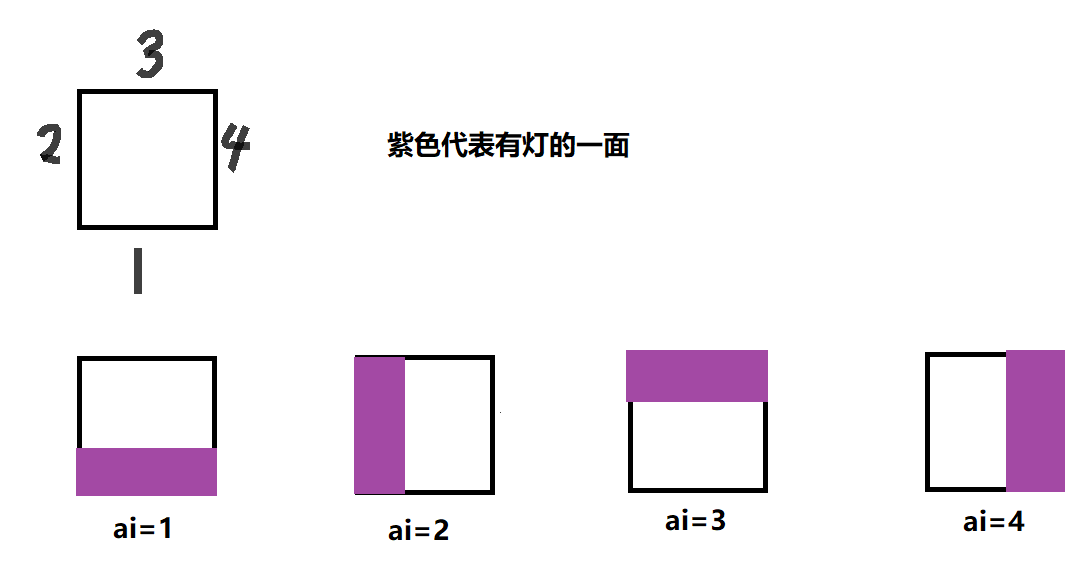
\includegraphics[scale=0.6]{./src/Problem-F-1.png}
\end{figure}

你的任务是转动每个柱子 $0$ 次或者若干次,使得正面全部朝向玩家($1$ 号面),输出任意一个可行解即可。

\subsection*{输入描述}

第一行是一个整数 $n$,表示正四棱柱的数量,$4 \leq n \leq 12$。

下一行是 $n$ 个整数,表示 $a_1, a_2, \dots, a_n$,其中 $1 \leq a_i \leq 4$。

第 $3$ 行到第 $n+2$ 行,每行有 $n$ 个整数($0$ 或 $1$)。第 $i+2$ 行的值表示 $b_{i,1}, b_{i,2}, \dots, b_{i,n}$ 的值,$b_{i,i}$ 总是为 $1$。

输入数据保证有解。

\subsection*{输出描述}

一行 $n$ 个整数,整数之间一个空格隔开,第 $i$ 个整数表示顺时针转动第 $i$ 个柱子多少次。允许的范围为 $0$ 到 $10^9$。如果存在多个解,请输出任意一个解。

\subsection*{测试样例}

\begin{table}[H]
\begin{tabularx}{\textwidth}{|X|X|}
    \hline
    \textbf{Standard Input} & \textbf{Standard Output} \\ 
    \hline
    \tablecell{
        4 \\
        4 2 1 2 \\
        1 0 1 0 \\
        0 1 1 0 \\
        0 0 1 0 \\
        1 0 0 1 \\
    } & \tablecell{
        2 3 3 3 \\ \\ \\ \\ \\ \\
    } \\
    \hline
\end{tabularx}
\end{table}

\subsection*{样例解释}

\begin{figure}[H]
    \centering
    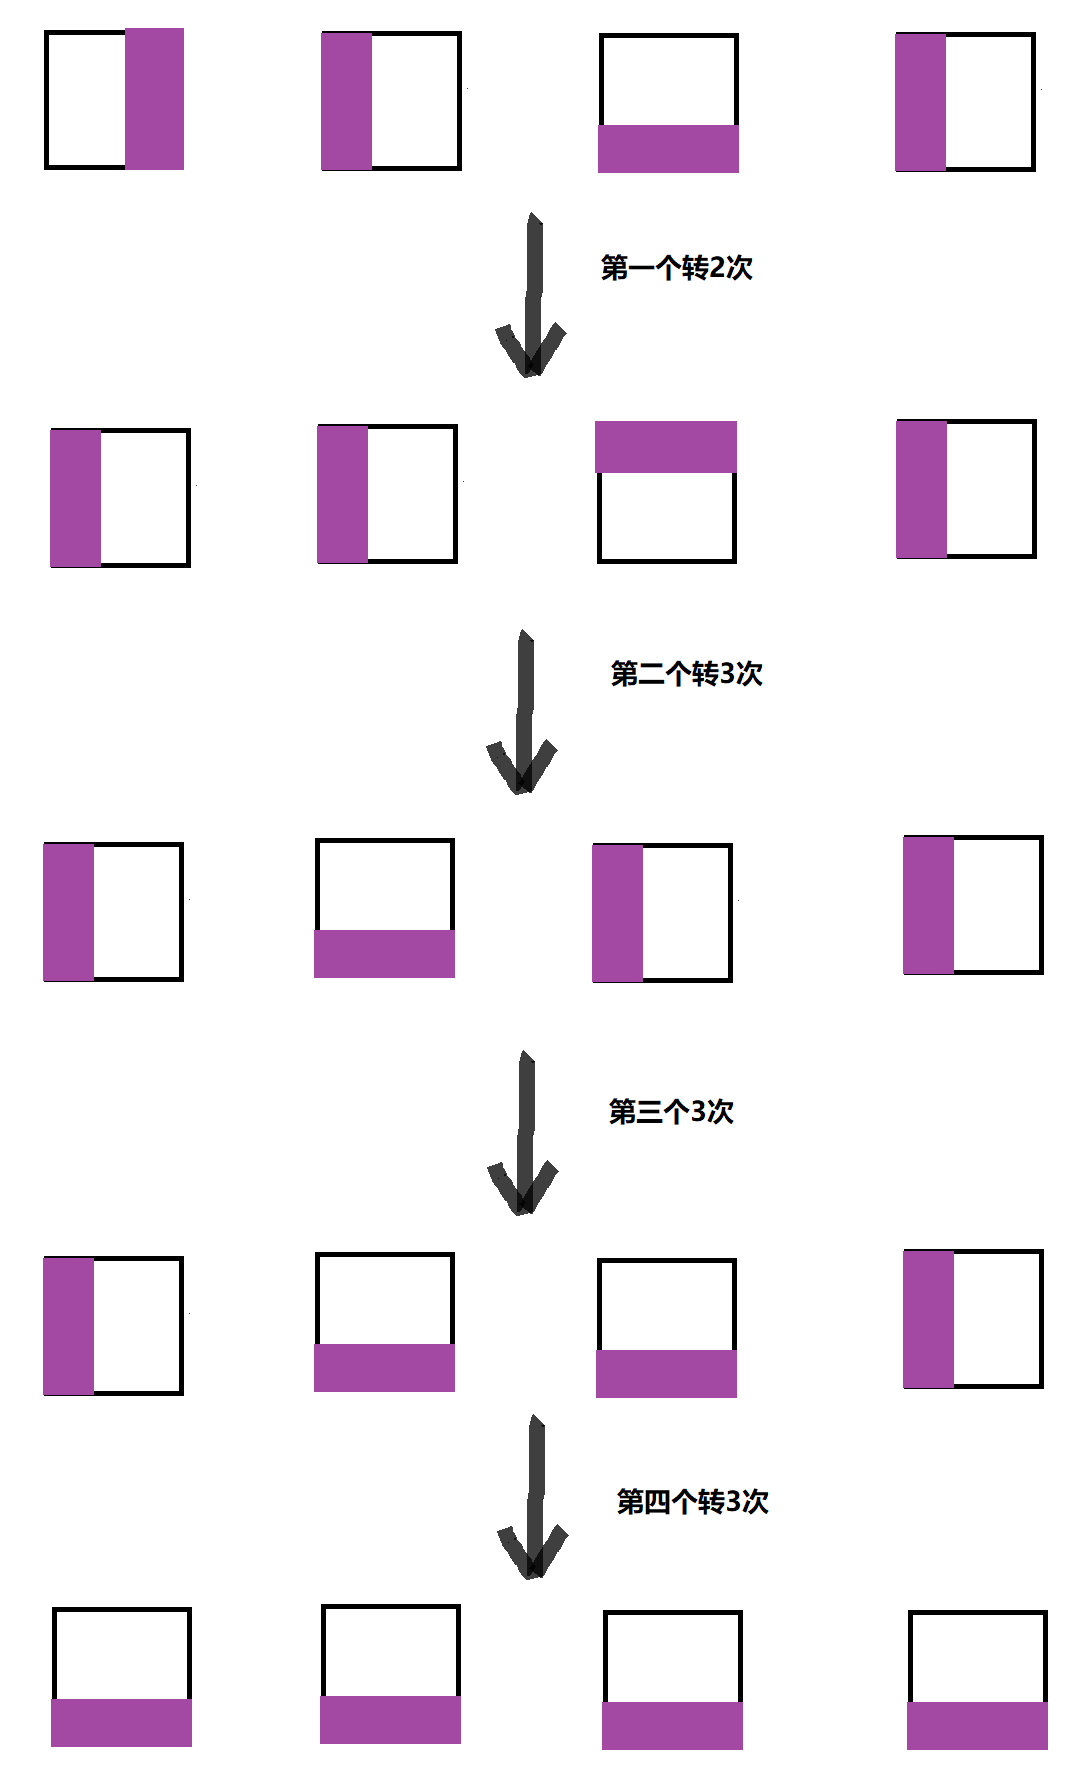
\includegraphics[scale=0.3]{./src/Problem-F-2.png}
\end{figure}